% vim: fileencoding=utf-8:tw=0:noexpandtab:ts=4:sw=4
% -*- coding: utf-8 -*-

\documentclass[letterpaper, 10pt, conference]{ieeeconf}

\IEEEoverridecommandlockouts
\overrideIEEEmargins
\pdfminorversion=4

% packages
\usepackage[mathletters]{ucs}
\usepackage[utf8x]{inputenc}
\usepackage{graphicx}
\usepackage{microtype}
\usepackage{amsmath}
\usepackage{url}
\usepackage{tabularx}

% options
\graphicspath{{figures/}{generated-figures/}}

% commands
\newcommand{\fig}[1]{Figure~\ref{fig:#1}}
\newcommand{\Fig}[1]{Figure~\ref{fig:#1}}
\newcommand{\tbl}[1]{{Table}~\ref{fig:#1}}
\newcommand{\Tbl}[1]{{Table}~\ref{fig:#1}}
\newcommand{\sect}[1]{Section~\ref{sec:#1}}
\newcommand{\Sect}[1]{Section~\ref{sec:#1}}
\newcommand{\hypo}[1]{Hypothesis~\ref{hyp:#1}}
\newcommand{\Hypo}[1]{Hypothesis~\ref{hyp:#1}}
\newcommand{\algo}[1]{Algorithm~\ref{algo:#1}}
\newcommand{\Algo}[1]{Algorithm~\ref{algo:#1}}
\newcommand{\eq}[1]{Equation~\ref{eq:#1}}
\newcommand{\Eq}[1]{Equation~\ref{eq:#1}}
\newcommand{\ent}[1]{\mathrm{H}_\mathrm{#1}} % entropy (\H already exists :/)

% title and authors

\title{\LARGE \bf
Localization of inexpensive robots with low-bandwidth sensors
}

\author{Shiling Wang$^{1}$ and Francis Colas$^{2}$ and Ming Liu$^{3}$ and Francesco Mondada$^{4}$ and Stéphane Magnenat$^{5}$% <-this % stops a space
\thanks{$^{1}$Shiling Wang is with ETH Zürich
        {\tt\small shilingwang0621@gmail.com}}%
\thanks{$^{2}$Francis Colas is with INRIA Nancy Grand Est
        {\tt\small francis.colas@inria.fr}}%
\thanks{$^{3}$Ming Liu is with City University of Hong Kong
        {\tt\small mingliu@cityu.edu.hk}}%
\thanks{$^{4}$Francesco Mondada is with Mobots, LSRO, EPFL
        {\tt\small francesco.mondada@epfl.ch}}%
\thanks{$^{5}$Stéphane Magnenat is with Mobots, LSRO, EPFL
        {\tt\small stephane@magnenat.net}}%
}

\begin{document}

\maketitle
\thispagestyle{empty}
\pagestyle{empty}

\begin{abstract}
Recent progress in electronics has allowed the construction of affordable mobile robots.
This opens many new opportunities, in particular in the educational context.
However, for cost reasons these robots have little long-range sensing abilities and bad dead-reckoning capabilities.
This limitation has prevented them from performing global localization without external aids.
This severely limits their use, for example to teach spatial reasoning or develop artistic activities.
In this paper, we propose a solution to this problem, using only infrared ground sensors, approximate dead-reckoning, and a visual pattern on the ground.
Our approach builds on a recursive Bayesian filter, of which we demonstrate two implementations: a dense Markov Localization and a particle-based Monte Carlo Localization.
We show that both implementations allow accurate localization on a large variety of patterns, from pseudo-random black and white matrices to grayscale drawings by children.
We demonstrate the real-time localization of a Thymio robot on these patterns.
These results show that by enabling a new range of educational activities, our solution to the localization of inexpensive robots strongly increases the value of robots for education.

\end{abstract}

\section{Introduction}

Driven by consumer products, the technologies of electronics, motor and battery have made tremendous progress in the last decades.
They are now widely available at prices making affordable mobile robots a reality.
This opens many new opportunities, in particular in the educational context.
Robots have been shown to be effective in supporting the teaching of knowledge in fields such as mathematics, physics, computer science and engineering; and of skills such as problem solving and introduction to the scientific method~\cite{benitti2012explorin, karim2015review}.

Programmable platforms in the 300--400\,\$ price range, such as the LEGO Mindstorms, have been successfully used in classrooms worldwide, especially to teach engineering.
% FIXME: fuzzy grammar in link
Yet, despite its high price tag, this platform has little perception capabilities: its longest-range sensor is a single ultrasound unit.
The much cheaper hobbyist mBot platform (75\,\$) is also equipped with a similar ultrasound device as its sole exteroceptive sensor.
Cheaper general public products such as the Thymio~II (130\,\$) and Dash \& Dot (160\,\$) even lack such long-range perception capability, and only provide local infrared sensors.
These are limited to sensing distances up to 15\,cm and measuring the grayscale intensity of a close object or the ground.
These products also lack a camera, because processing images would require extended memory and processing resources, which would increase their price significantly.
Therefore, all affordable general-public educational robots (in the 100\,\$ range) lack long-range sensing capabilities.
In addition, dead-reckoning on these platforms is bad to non-existent.
An exception is the BeeBot (90\,\$), which uses proper dead-reckoning as its only sensor, and so has only a narrow set of possible use.
On platforms that must already provide a variety of programming and sensing modalities to meet general educational needs, proper wheel encoders are still too expensive.
Hence when dead-reckoning is provided, such as on the Thymio~II, it builds on approximate methods such as measuring the back electromotive force.

% But this robot can only follow pre-programmed trajectories, it is not able to react to external events.

\begin{figure}
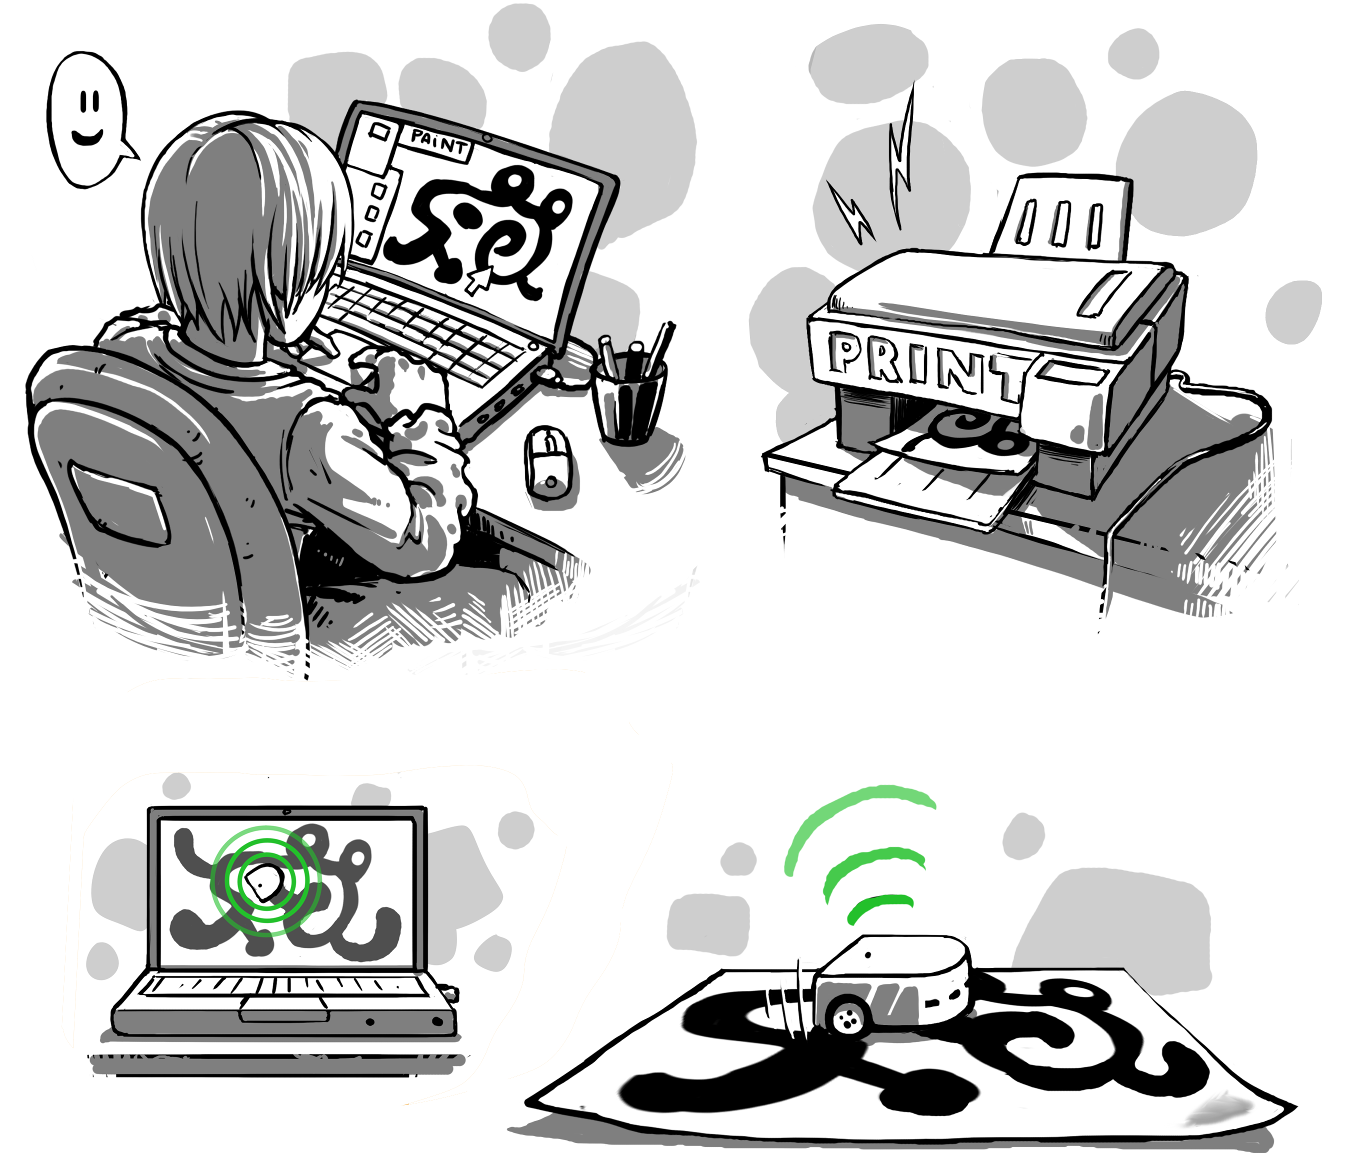
\includegraphics[width=\columnwidth]{process_creation_col_small}
\caption{The process of creating a ground drawing serving as the map.}
\label{fig:process}
\end{figure}

The combined lack of long-range sensors and poor quality dead-reckoning prevents affordable educational robots from using state of the art localization algorithms such as simultaneous localization and mapping.
This lack of absolute positioning hinders their educational use, especially with constructivist or constructionist approaches (the most commons in robot-based educational material), because spatial reasoning has been recognized as a critical element for learning about the world~\cite{lesh2003beyond}.
This has negative effects for the study of geometry, physics, and engineering;
In addition, while robots have the potential to reach minorities currently under-represented in technical fields, they typically do so through art and storytelling~\cite{szecsei2015girls}.
Such educational activities, for example staging a theater play with robots, would typically benefit from having absolute positioning.

This paper answers this need by providing an absolute positioning system using only approximate dead-reckoning and inexpensive infrared sensors measuring the grayscale intensity of the ground, without knowing the initial pose of the robot.
The ground can be an existing image or a drawing created by the child herself (\fig{process}).
Our solution is based on the classical Markov~\cite{fox1999markov} and Monte Carlo~\cite{dellaert1999monte} Localization frameworks that can be seen as respectively a dense and a sampling-based implementation of a recursive Bayesian filter.
While these approaches are commonly deployed in robots with extensive sensing capabilities such as laser scanners, their implementation on extremely low bandwidth sensors is novel, and rises specific questions, such as which distance the robot must travel for the localisation to converge.
%Our solution builds on a recursive Bayesian filter, of which we propose both a dense and a sampling-based implementation.
% FIXME: improve link
We evaluate these using the Thymio~II mobile robot on a known black and white pseudo-random pattern, with ground truth provided by a Vicon tracking system.
In addition, we provide a theoretical contribution predicting the traveled distance necessary to localize the robot.
Finally, we show how grayscale images can be used as ground patterns that allow the robot to localize.
% FIXME: rewrite, highlight final process

\section{Related work}

The main challenge of solving the localization problem on affordable mobile robots is the limited information content typical inexpensive sensors can provide.

Zug et al.~\cite{zug2011design} have developed an algorithm using an array of triangulation-based infrared distance sensors.
A Kalman filter algorithm is applied to localize the robot within a 2 by 1\,m box.
No experimental result is provided, but a simulation shows the estimated error to be within 2\,cm.
Pinto et al.~\cite{pinto2012localization} have developed a localization system using only one of these sensors, in the context of education.
They mount the sensor on a platform built around a LEGO Mindstorms NXT and use an Extended Kalman Filter for localization.
However, they do not provide experimental result either.

Focusing on a low cost, Gutmann et al.~\cite{gutmann2013challenges} have developed a system using only 3 or 4 light detectors, able to localize a mobile robot in a room with an accuracy of 10\,cm.
Their system is based on detecting a known pattern projected on the ceiling and fusing this information with odometry.
However, this method demands the installation of a projector and requires empty space over it.

Park and Hashimoto~\cite{park2009approach} proposed to localize a mobile robot over a ground equipped with randomly distributed passive \textsc{rfid} tags.
The average localization error of this method is lower than 10\,cm.
However, this approach requires the ground to be equipped, and is only applicable when the starting position of the robot is known.

In the context of education, Singh and Bedi~\cite{singh2013map} have used the ultrasound sensor of the LEGO Mindstorms NXT to localize a robot in a room.
They use a Monte Carlo Localization approach based on a particle filter.
However, they do not provide quantitative results.

Dias and Ventura~\cite{dias2013absolute} use two horizontal lines from a \textsc{vga} camera to read barcodes on the walls of an arena and localize an e-puck robot.
Their system employs an Extended Kalman Filter algorithm and reaches a precision of 1\,cm and 5°.
As with the work of Singh and Bedi, it requires an enclosed arena with a specific wall arrangement and no obstacles between the robot and the walls.

Another line of research has approached the localization problem by using multiple robots and combining their perception.
Prorok et al.~\cite{prorok2012low} is representative of this approach.
These authors have used an infrared-based range and bearing hardware along with a distributed Monte Carlo Localization approach, allowing a group of robots to localize down to a precision of 20\,cm.
However, this line of research focuses on scalability rather than absolute positioning, as the later would require fixed robots acting as beacons.
In addition, both radio and infrared-based range and bearing systems require complex electronics.
Finally, when the cost of all robots is added, the system is far from cheap.

To the best of our knowledge, there exist no onboard localization system able to use a low number of\,--\,or a single\,--\,inexpensive local infrared sensor(s), and able to provide absolute positioning in a distributed way.
The system proposed in this paper meets these requirements.

\section{Material}
\begin{figure}
\raisebox{.3cm}{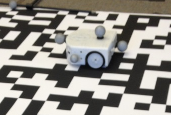
\includegraphics[width=.53\columnwidth]{thymio2-dataset}}\hfill
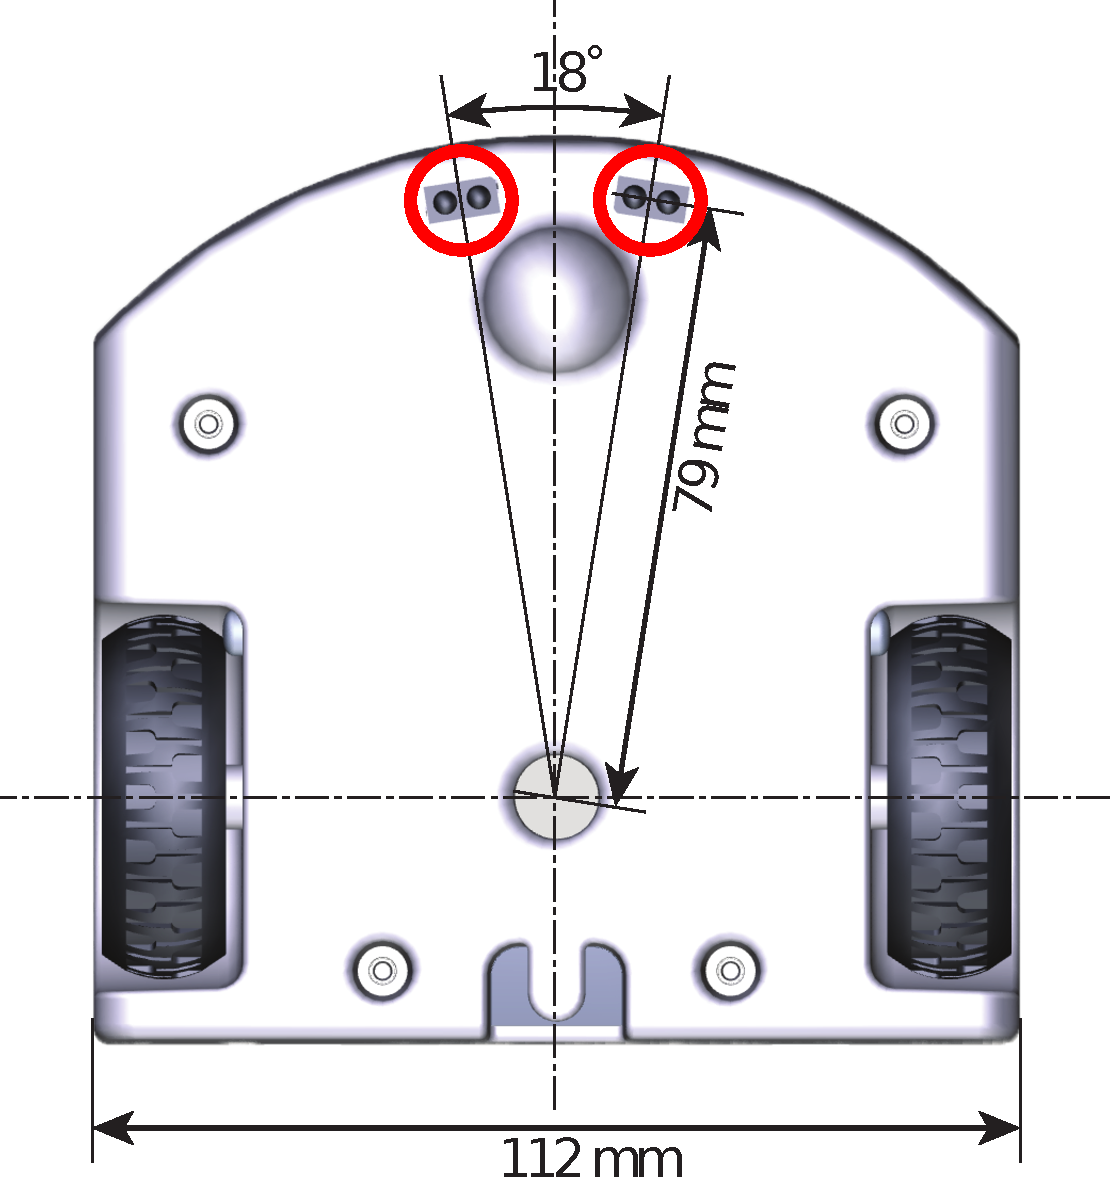
\includegraphics[width=.43\columnwidth]{thymio2-dimensions}
\vspace{-.07cm}
\caption{The Thymio~II robot with markers for tracking its ground-truth pose by a Vicon system (left), and the placement of its ground sensors (right).}
\label{fig:thymio}
\end{figure}

We run empirical experiments with the Thymio~II mobile robot localizing on a printed pattern, which forms its map.

Thymio~II is an open-source differential-wheeled mobile robot (\fig{thymio}).
Its footprint is approximately $10 \times 10$ cm and it costs about 130\,\$.
Thousands of units have been sold to date and are used in the context of computational thinking and engineering education~\cite{riedo2015thymio}.
It features many sensors such as a set of infrared sensors, a small accelerometer, and a microphone.
This project uses only its two ground infrared sensors (\fig{thymio}, right, circled red) and the measurement of the back electromotive force, which is proportional to the speed of the wheels.
Thymio~II is programmed through the \textsc{aseba} framework~\cite{aseba2011tmech}, which connects to \textsc{ros}\footnote{ROS (Robot Operating System): \url{http://www.ros.org/}}.

To evaluate the performance of our localization algorithms, we create datasets.
The robot moves with a speed of 3--5\,cm/s on a 150$\times$150\,cm ground pattern containing 50\,$\times$\,50 cells of 3$\times$3\,cm, each randomly black or white (\fig{thymio}, left).
We record the ground-truth pose of the robot using a Vicon\footnote{\url{http://www.vicon.com/}} tracking system.
%to provide the ground-truth robot pose, consisting of $x$, $y$ coordinates and the heading $\theta$.
We use \textsc{ros} to synchronously record these along with sensor values and odometry information from Thymio.
The data are gathered with a frequency of 100\,Hz (ground-truth) and 10\,Hz (robot) and subsequently down-sampled to a period of 0.3\,s.
We chose this period so that at maximum speed, the robot travels approximately half the length of one cell between every sample.
The motions of the robot can be classified into two different types, namely moving forward or backward (possibly in arcs) and rotating on spot.
To fully explore the performance of the algorithm, we remotely control the robot along several trajectories covering all possible motions.
To test the algorithm's ability of recovering from catastrophic localization failures, we also conduct experiments with ``robot kidnapping'' by lifting the robot and moving it to another part of the map.

% TODO: add protocol for the final experiment

\section{Model}

% FIXME: this hat can be compressed...

In this section, we start by presenting the generic Bayesian filter used to estimate the pose of the robot in the environment.
Then we discuss the specificities of the Markov Localization and Monte Carlo Localization approaches for its inference.
Finally, we propose a theoretical analysis from an information theoretic point of view to give a lower bound on the time or distance to start achieving localization.

\subsection{Pose estimation filter}
%\subsection{Variables}

The generic model uses the following variables:
\begin{itemize}
\item $X_{1:t}$ 2-D pose at times $1..t$.
The pose vector consists of $x,y$ coordinates and an angle $\theta$.
\item $Z_{1:t}$ observations at times $1..t$.
The observation consists of the output of two sensors located at the bottom of the robot, measuring the grayscale intensity of the ground.
\item $U_{1:t}$ odometry at times $1..t$.
The odometry consists of the left and right wheel speeds.
\end{itemize}

%\subsection{Joint probability}
It is classically formulated as a recursive Bayesian filter with the following joint probability distribution:
\begin{equation*}
\begin{split}
& p(X_{1:t}, Z_{1:t}, U_{1:t}) = \\
& p(Z_t|X_t) p(X_t|X_{t-1}, U_{t}) p(U_t) p(X_{1:t-1}, Z_{1:t-1}, U_{1:t-1}).
\end{split}
\end{equation*}

%\subsection{Question}
This joint probability distribution allows to formulate the problem as the estimation of the pose $X_t$ at time $t$ given the observations $Z_{1:t}$ and the commands $U_{1:t}$:
\begin{equation*}
\begin{split}
& p(X_t|Z_{1:t},U_{1:t}) = \frac{p(X_t,Z_t | Z_{1:t-1}, U_{1:t})}{p(Z_t|Z_{1:t-1}, U_{1:t})} \\
% &\propto p(Z_t | X_t) p(X_t | Z_{1:t-1}, U_{1:t}) \\
% &\propto p(Z_t | X_t) \sum_{X_{t-1}} p(X_t, X_{t-1} | Z_{1:t-1}, U_{1:t} ) \\
 &\propto p(Z_t | X_t) \sum_{X_{t-1}} p(X_t|X_{t-1}, U_t) p(X_{t-1} | Z_{1:t-1}, U_{1:t-1}).
\end{split}
\end{equation*}
%This is a recursive filter to estimate $X_t$ using the previous estimation $X_{t-1}$, the odometry $U_t$ and the observation $Z_t$.

%\subsection{Distributions}
This inference involves the two distributions to specify, the \emph{observation model} $p(Z_t | X_t)$ and the \emph{motion model} $p(X_t|X_{t-1}, U_t)$.

\subsubsection{Observation model}

The robot has two infrared ground sensors measuring the grayscale value of the ground.
Despites the observations being coupled through the known map, our model assumes them to be independent, so $p(Z_t | X_t) = \prod_{i=0,1} p(Z_t^{i} | X_t)$.
Moreover, we assume the ground color to be in the range $[0,1]$ with $0$ being black and $1$ being white.
Hence, if sensor $i$ for robot pose $X_t$ should see a ground intensity $v$ according to the map, $p(Z_t^{i} | X_t) \sim \mathcal{N}(v,\sigma_\mathrm{obs})$.
The parameter $\sigma_\mathrm{obs}$ is selected based on the knowledge of the sensor.
For black and white patterns, we set it to $0.5$, giving a probability of $p_\mathrm{correct} = 0.95$ when the value measured by the sensor corresponds to the one in the map.
For grayscale images, based on measurement on a real Thymio, we set it to $0.1$.

\subsubsection{Motion model}

Based on the model of Eliazar et al.~\cite{eliazar2004motionmodel}, we assume that the motion has a Gaussian error model, hence $p(X_t~|~X_{t-1}, U_{t})\sim\mathcal{N}(\mu_t,\Sigma_t)$.
The mean $\mu_t$ is built by accumulating the estimated displacements by dead-reckoning between times $t-1$ and $t$.
Therefore, if $\Delta x_t$, $\Delta y_t$, $\Delta \theta_t$ are the displacement between $t-1$ and $t$, expressed in the robot local frame at $t-1$, $\mu_t$ is:
\begin{equation*}
\mu_t =
\left[ \begin{array}{c} x_t \\ y_t \\ \theta_t \end{array} \right]
\text{with}
\begin{array}{c}
\left[ \begin{array}{c} x_t \\ y_t \end{array} \right] =
\left[ \begin{array}{c} x_{t-1} \\ y_{t-1} \end{array} \right] +
R(\theta_{t-1})
\left[ \begin{array}{c} \Delta x_{t} \\ \Delta y_{t} \end{array} \right]
\\
\theta_t = \theta_{t-1} + \Delta \theta_t
\end{array}
\end{equation*}
where $R(\theta)$ is the 2-D rotation matrix of angle $\theta$.
The $3\times3$ diagonal covariance matrix $\Sigma_t$ is a function of the distance traveled, the amount of rotation, and two parameters $\alpha_\mathrm{xy}$, $\alpha_\theta$:
\begin{equation*}
\Sigma_t=\begin{bmatrix} \sigma_{\mathrm{xy},t}^2 & 0 & 0 \\ 0 & \sigma_{\mathrm{xy},t}^2 & 0 \\ 0 & 0 & (\alpha_\theta | \Delta \theta_t |)^2 \end{bmatrix}
\end{equation*}
with $ \sigma_{\mathrm{xy},t} = \alpha_\mathrm{xy} \sqrt{\Delta x_{t}^2 + \Delta y_{t}^2}$.

In addition, to cope for the possibility of the robot being kidnapped and therefore its pose becoming unknown, a uniform distribution with a weight $p_\mathrm{uniform}$ is added to $X_t$.

The parameters $\alpha_\mathrm{xy}$, $\alpha_\theta$ and $p_\mathrm{uniform}$ are estimated using maximum likelihood (see \sect{mle}).

\subsubsection{Self confidence}

We define a self-confidence term that corresponds to the ratio of the probability mass of $p(X_t)$ that is within a distance $d_\mathrm{xy}$ and an angle difference $d_\theta$ to the mode.
In the result section, we use $d_\mathrm{xy} = 3$\,cm and $d_\theta = 10$°.

\subsection{Implementations}

We compare two variants of this filter.
In Markov Localization, the distributions are discretized using regular grids~\cite{fox1999markov}.
For our experiments, the $x,y$ cell resolution is 1\,cm and the angular resolution varies from 20° (18 discretization steps for 360°) to 5° (72 discretization steps for 360°).

In Monte Carlo Localization~\cite{dellaert1999monte}, the distributions are represented using samples in a particle filter.
In order to extract a single pose estimate out of the many particles, we find a maximum density area in which we average the particles.
It is similar to a 1-point \textsc{ransac} scheme~\cite{Fischler1981ransac}.
%Both the search for the particle with most neighbors and the search for neighbors are done with 500 trials.
%The thresholds for a particle to be a neighbor are a distance of 1.5\,cm and an angular difference of 5°.

We implemented both algorithms in Python with some Cython\footnote{\url{http://www.cython.org}} procedures used for time-critical inner loops.

\subsection{Theoretical analysis of convergence}
\label{sec:theoreticalconv}

It is possible to estimate the time required for the robot to localize itself in a given known space.
For the Markov Localization approach, there is a given number of discrete cells.
The amount of information needed to unambiguously specify one among them all is $\ent{loc} = \log_2(N_\mathrm{cells})$, with $N_\mathrm{cells}$ the number of cells.

We can also compute the information gain at each time step.
Indeed, a binary sensor ideally yields 1\,bit of information per measurement.
However in practice, there is a loss in information due to the sensor noise, characterized by the $p_\mathrm{correct}$ probability of the sensor to be correct:
\begin{displaymath}
	\ent{noise} = \ent{b}(1 - p_\mathrm{correct}),
\end{displaymath}
where $\ent{b}$ is the binary entropy function: $\ent{b}(p) = -p\log_2(p) - (1-p)\log_2(1-p)$.

In addition, we need to take into account that our sensor measurements are not completely independent.
For example, when not moving, we always observe the same place and thus cannot really gain additional information besides being sure of the intensity of the current pixel.
In a discretized world, we thus need to estimate the probability of having changed cell in order to observe something new, which depends on the distance traveled and the size of the cells.
This problem is equivalent to the Buffon-Laplace needle problem of finding the probability for a needle thrown randomly on a grid to actually intersect the grid~\cite{laplace1820prob}.
In our case, the probability of changing cell is given by:
\begin{displaymath}
	p_\mathrm{diff} = \frac{4d h - d^2}{\pi h^2},
\end{displaymath}
with $d$ the distance traveled and $h$ the size of the cells.

We can then compute the conditional entropy for two successive ideal measurements separated by $d$ based on the conditional probability:
\begin{align*}
	&P(O_t | O_{t-1})\\
	&= \begin{pmatrix}
		(1 - p_\mathrm{diff}) + 1/2 p_\mathrm{diff} & 1/2 p_\mathrm{diff}\\
		1/2 p_\mathrm{diff} & (1 - p_\mathrm{diff}) + 1/2 p_\mathrm{diff}
	\end{pmatrix}.
\end{align*}
Therefore the loss of information due to redundancy in the travelled distance is:
\begin{displaymath}
	\ent{loss,d} = 1 - \ent{b}(1/2 p_\mathrm{diff}).
\end{displaymath}

There is also redundancy between several sensors placed on the same robot.
The probability that they see the same cell based on the distance between them is exactly the same as the probability of a sensor to see the same cell after a displacement of the same distance.
The information loss due to the redundancy from the sensor placement is noted $\ent{sensors}$ and follows the same formula as $\ent{loss,d}$ for the given distance.

Finally, we can approximate the information that our robot gathers at each time step in the following manner:
\begin{align*}
	&\ent{}(O^1_t, O^2_t | O^1_{1:t-1}, O^2_{1:t-1})\\
	&= \ent{}(O^1_t, O^2_t | O^1_{t-1}, O^2_{t-1}) \\
	&= \ent{}(O^1_t | O^1_{t-1}) + \ent{}(O^2_t | O^2_{t-1}) - \ent{}(O^2_t | O^1_t) \\
	&= 2*(1-\ent{noise}-\ent{loss,d}) - \ent{sensors}%. The full stop here is ugly.
\end{align*}
This approximation assumes that the trajectory of the robot is ideal (no longer time redundancy) and that the trajectories of the sensors are independent.
It also ignores the uncertainty in the robot motion.
As such, it is therefore an upper bound on the average information gain.

In our example, we have assumed $p_\mathrm{correct}=0.95$, that is $\ent{noise}=0.29$.
Our robot moves at 3\,cm/s with a time step of 0.3\,s and 3\,cm cells in which the color is know to be similar; this yields $p_\mathrm{diff}=0.35$ and $\ent{loss,d}=0.33$.
Finally the sensors are 2.2\,cm apart which yields $p_\mathrm{diff}=0.76$ and $\ent{sensors}=0.041$.
As such the robot gathers on average at most 0.72\,bit per time step, or 0.8\,bit/cm.

With a 150\,cm$\times$150\,cm environment discretized with cells of 1\,cm and 5° angle, the amount of information needed for the localization is $\ent{loc}=20.6$.
This means that, on average, the robot should not be localized before traveling around 26\,cm.

Faster localization can be achieved by moving at a greater speed to reduce redundancy in the successive measurements.
If designing a new robot, better sensors would reduce cross-over noise.
Setting the sensors apart would also reduce the redundancy between their information but, for our specific grid size, they are sufficiently separated in Thymio~II.

\section{Experiments}

\subsection{Dataset collection}

\begin{figure}
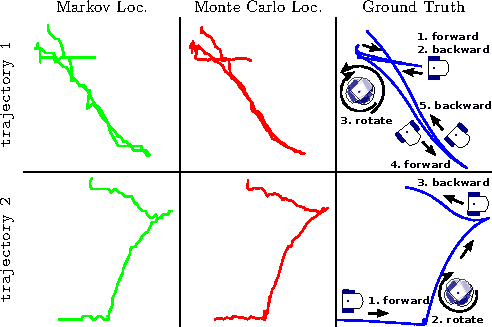
\includegraphics{trajectories}
\caption{The estimations (after convergence) along with the ground truth for the two first trajectories.
For Markov Localization, the angle discretization is 72; for Monte Carlo Localization, there are 400k particles.
}
\label{fig:trajectories}
\end{figure}

Our experiments are based on four datasets:
\begin{itemize}
\item \texttt{trajectory 1} and \texttt{2}: The robot alternates forward and backward movements with rotations on spot;
\item \texttt{trajectory with kidnapping}: The robot alternates phases of forward movement and turning on spot, with kidnapping happening every minute;
\item \texttt{linear trajectory}: The robot simply goes straight ahead along the x-axis of the map.
\end{itemize}
\Fig{trajectories} shows the estimated trajectories for the first two runs using the two variants of the filter.

\subsection{Parameter estimation}
\label{sec:mle}

The noise parameters of the motion model were estimated using maximum likelihood, considering the error between the ground truth and the odometry data in the local frame between two time steps.
Using \texttt{trajectory~1} and \texttt{trajectory~2}, the values for  $\alpha_\mathrm{xy}$ and $\alpha_\theta$ were found be in the order of 0.1.
Similarly, using \texttt{trajectory with kidnapping}, the value for $p_\mathrm{uniform}$ was also found to be in the order of 0.1.

\subsection{Basic localization}

\begin{figure*}

\begin{center}
Markov Localization, \texttt{trajectory~1}, for different \emph{number of discretization angles}
\end{center}
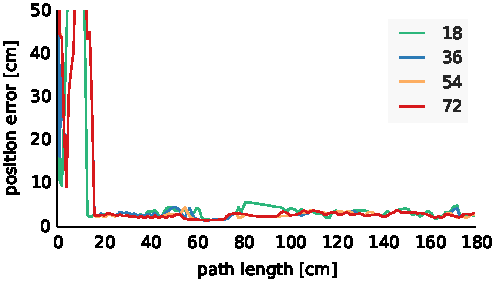
\includegraphics{ml-whole_random_1-xy}\hfill
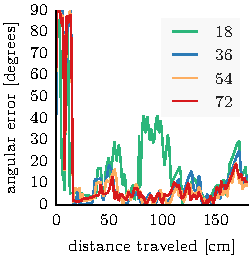
\includegraphics{ml-whole_random_1-theta}

\vspace{.3em}

\begin{center}
Markov Localization, \texttt{trajectory~2}, for different \emph{number of discretization angles}
\end{center}
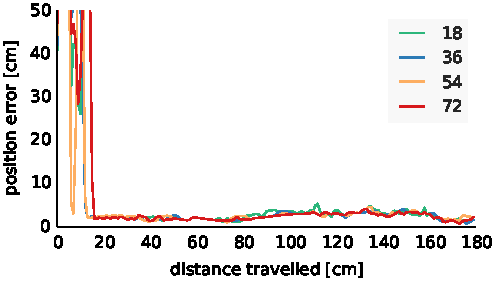
\includegraphics{ml-whole_random_2-xy}\hfill
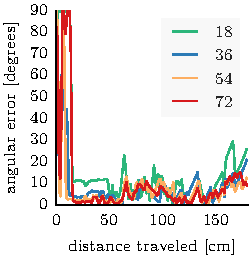
\includegraphics{ml-whole_random_2-theta}

\vspace{.3em}

\begin{center}
Monte Carlo Localization, \texttt{trajectory~1}, for different \emph{number of particles}
\end{center}
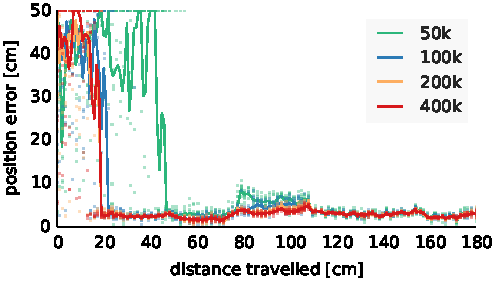
\includegraphics{mcl-whole_random_1-xy}\hfill
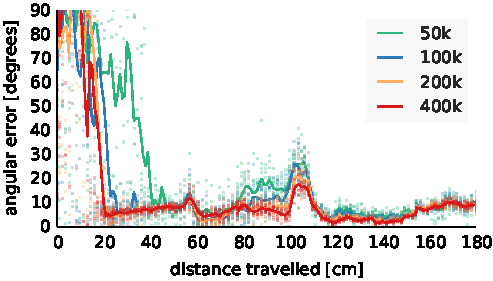
\includegraphics{mcl-whole_random_1-theta}

\vspace{.3em}

\begin{center}
Monte Carlo Localization, \texttt{trajectory~2}, for different \emph{number of particles}
\end{center}
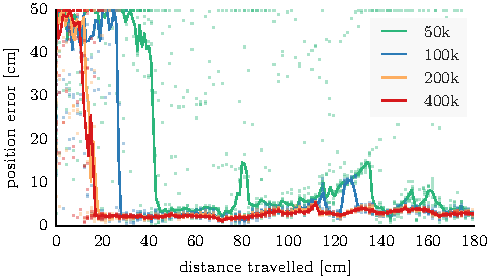
\includegraphics{mcl-whole_random_2-xy}\hfill
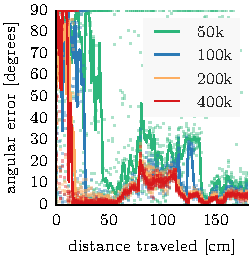
\includegraphics{mcl-whole_random_2-theta}

\caption{The error between the estimation by the localization algorithm and the ground truth on \texttt{trajectory~1} (top) and \texttt{trajectory~2} (bottom).
For Monte Carlo Localization, the solid lines show the average over 10 trials, while the light dots show the individual trials.}
% FIXME: I (Steph) is not convinced the legend is correct
\label{fig:whole-runs-random12}
\end{figure*}

\Fig{whole-runs-random12} shows the error in position and orientation for the first two trajectories.
In these plots, \emph{distance traveled} represents the cumulative distance traveled by the center point between the two ground sensors of the robot.
The error is clamped at 50\,cm for position and 90° for orientation.

For Markov Localization approach, all discretization resolutions allow the robot to localize with a precision of 3\,cm and 5°.
In \texttt{trajectory~1}, the resolution of 18 discretization steps is not enough to keep tracking the orientation at a distance traveled of 50\,cm and 80\,cm.
These both correspond to the robot rotating on spot.
We see that an angular discretization of 36 (10° resolution) is sufficient to provide accurate tracking, and that a finer resolution only provides minor improvements in angular precision, and no improvement in position precision.
In \texttt{trajectory~2}, we see that a resolution of 54 allows for a better angular precision than 36, but 72 does not improve over 54.
All resolutions provide equal position precision.

For Monte Carlo Localization approach, we see that on \texttt{trajectory~1}, the robot localizes already with 50k particles, but in twice the time it takes with 100k particles.
Increasing the number of particles beyond this value only marginally decreases localization time.
While 50k particles are sufficient to localize on this run on average, in some runs, the robot looses orientation, when it turns on spot.
On \texttt{trajectory~2}, 50k particles is not enough to localize the robot.
Increasing this number to 100k leads to a good localization, except after the robot has traveled 80\,cm; which corresponds to a long moment during which the robot rotates on spot, leading to less information acquisition, and therefore degraded precision.

Overall, both approaches have similar localization accuracy.
When angular precision is critical, the Monte Carlo Localization approach might achieve better performance, as the Markov Localization approach is limited in precision by its discretization.
%FIXME: move this into conclusion

%TODO: explain why this does not appear in ML

\subsection{Distance to converge}

\begin{figure}

\begin{center}
Markov Localization, 10 segments from the first two trajectories, for different \emph{number of discretization angles}
\end{center}
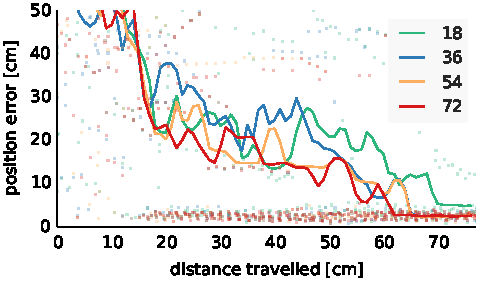
\includegraphics{ml-small_runs_random_12-xy}

\vspace{.3em}

\begin{center}
Monte Carlo Localization, 10 segments from the first two trajectories, for different \emph{number of particles}
\end{center}
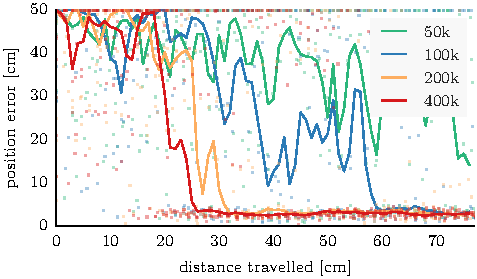
\includegraphics{mcl-small_runs_random_12-xy}

\caption{
The error between the estimation by the localization algorithm and the ground truth on 10 segments from the first two trajectories.
The solid lines show the median while the light dots show the individual trials.}
\label{fig:small-runs}
\end{figure}

\Fig{small-runs} shows the error in position for 5 different locations in the two first trajectories.
We see that, with the Markov Localization approach, the correct pose is found after about 20\,cm.
% TODO check that
%This corresponds well to the ideal theoretical distance of 18\,cm computed in \sect{theoreticalconv}.
This is shorter than the 26\,cm distance computed in \sect{theoreticalconv}.
This is probably due to the overestimation of the cross-over noise of the sensor.
A distance of 20,cm would correspond to noise lower than 3\% instead of 5\% as assumed.
% end TODO
There are also outliers: this happens when the robot is turning on spot, in which case there is not enough information to localize the robot.
The convergence is slower with Monte Carlo Localization approach, except with 400k particles, in which case it is roughly similar.
Decreasing the number of particles quickly increases the distance needed for convergence, reaching 60\,cm for 100k particles.
Using only 50k particles, some trajectory segments fail to converge, even after 80\,cm length.

\Fig{small-maps} shows the effect on convergence distance when the map size is reduced.
The robot runs linearly on one quarter of the map, while the Markov Localization is provided with the whole map, half of it, and a quarter of it.
We see that reducing the map size does reduce the distance traveled necessary to converge, in accordance to the theory.

\begin{figure}
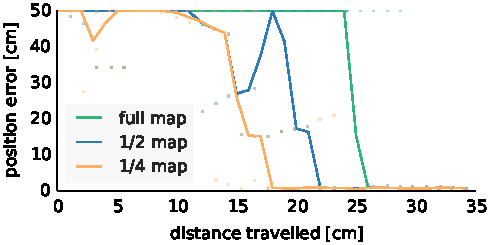
\includegraphics{ml-small_maps-xy}
%\vspace{.5em}
%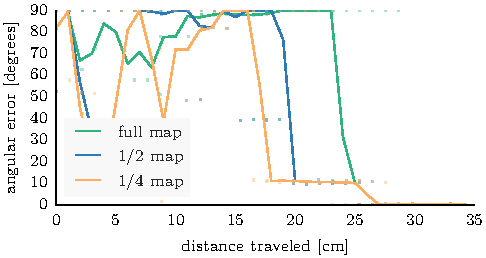
\includegraphics{ml-small_maps-theta}
\caption{The error between the estimation by the localization algorithm and the ground truth, using Markov Localization, for different map sizes on \texttt{linear trajectory}.
The solid lines show the median over 3 different sizes, while the light dots show the individual sizes.}
\label{fig:small-maps}
\end{figure}

\subsection{Robot kidnapping}

\begin{figure}

\begin{center}
Markov Localization, \texttt{trajectory with kidnapping}, for different \emph{number of discretization angles}
\end{center}
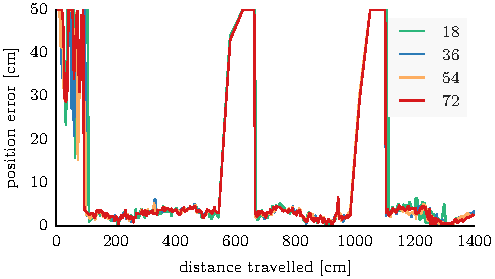
\includegraphics{ml-whole_random_long-xy}

\vspace{.3em}

\begin{center}
Monte Carlo Localization, \texttt{trajectory with kidnapping}, for different \emph{number of particles}
\end{center}
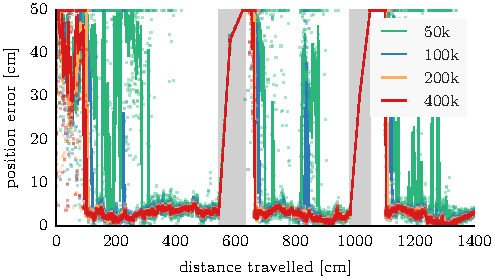
\includegraphics{mcl-whole_random_long-xy}

\caption{The error between the estimation by the localization algorithm and the ground truth on the run with kidnapping.
For Monte Carlo Localization, the solid lines show the median over 10 trials, while the light dots show the individual trials.
The gray areas show the time during the robot is being held in the air at the occasion of kidnapping.}
\label{fig:whole-runs-random-long}
\end{figure}

\Fig{whole-runs-random-long} shows the error in position for the run with kidnapping.
In this run, the robot is kidnapped twice, after having traveled 550\,cm and 1000\,cm.
It takes the robot approximately 50\,cm to re-localize, and does so successfully with both Markov and Monte Carlo Localization approaches.
% FIXME: check on the video for numbers, edit plots
With Markov Localization approach, discretization resolutions of 36, 54 and 72 are approximately equivalent in performance, while 18 performs clearly worst, but only for angular resolution.
With Monte Carlo Localization approach, the robot localizes most of the time with 100k particle or more, and always with 200k particles or more.
With 50k particles, the robot eventually localizes, but this might take more than 2 meters of traveled distance.
%TODO: reanalyse MCL once we have 10 runs
%FIXME: make more clear

\subsection{Computational cost}

\begin{figure}
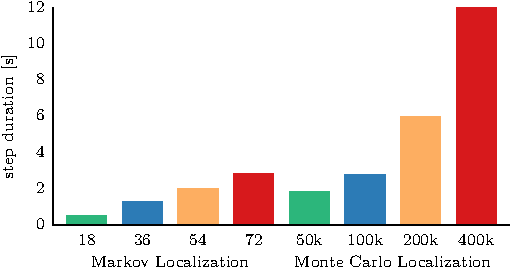
\includegraphics{cpu_load}
\caption{The execution duration, proportional to the computational cost, for one time step.
For Markov Localization, the legend indicates the number of discretization steps for angles; for Monte Carlo Localization, the number of particles.
Data are averaged over all time steps of first two trajectories.}
\label{fig:cpuload}
\end{figure}

\Fig{cpuload} shows the duration of one step for the different algorithms and parameters, averaged over the two first trajectories.
These data were measured on a Lenovo laptop T450s with an Intel Core i7 5600U processor running at 2.6\,GHz.
We see that with the Markov Localization approach, the duration scales linearly with the number of discretization angles.
With the Monte Carlo Localization approach, the scaling is linear but amortized (50k particles is not twice faster as 100k).
This is due to the selection of pose estimate, which uses a \textsc{ransac} approach and is therefore independent of the number of particles.
For similar localization accuracy, the Monte Carlo Localization approach is slower than the Markov Localization approach, and therefore we suggest to use the former with a discretization angle of 36 in practical applications.
However, the Monte Carlo Localization approach might be preferred if a high angular precision is required.
%FIXME: move this into conclusion

At a computation duration of 1.5\,s per step, the Monte Carlo Localization approach with a discretization angle of 36 is far from real time.
However, this computation duration corresponding to a map size of 150\,cm.
If the map was smaller, for instance 50\,cm, the algorithm would be 9 times faster.
Therefore, at 0.15\,s per step, it would be suitable for real-time operations.
Moreover, the code could be further optimized by using multimedia instructions such as \textsc{sse}, implementing it in the \textsc{gpu}, or parallelizing it.
Conditional probability tables are well suited for such optimizations.
The Monte Carlo Localization approach requires at least 100k particle for proper localization, at a computation duration of 2\,s per step.
While similar optimization is possible, some parts are harder to optimize, in particular the re-sampling step and the \textsc{ransac} step.
% FIXME: implement real-time and get rid of this last paragraph

\subsection{Grayscale images as maps}

\begin{figure*}
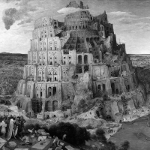
\includegraphics[width=.15\textwidth]{maps/breugel_babel} \hfill
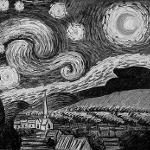
\includegraphics[width=.15\textwidth]{maps/van-gogh_starry-night} \hfill
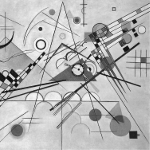
\includegraphics[width=.15\textwidth]{maps/kandinsky_comp-8} \hfill
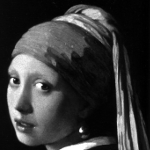
\includegraphics[width=.15\textwidth]{maps/vermeer_girl-pearl} \hfill
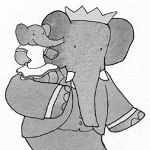
\includegraphics[width=.15\textwidth]{maps/babar} \hfill
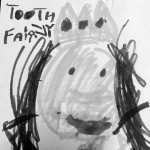
\includegraphics[width=.15\textwidth]{maps/childs-drawing_tooth-fairy}

\makebox[.15\textwidth][c]{Breugel}\hfill
\makebox[.15\textwidth][c]{Van Gogh}\hfill
\makebox[.15\textwidth][c]{Kandinsky}\hfill
\makebox[.15\textwidth][c]{Vermeer}\hfill
\makebox[.15\textwidth][c]{Babar}\hfill
\makebox[.15\textwidth][c]{Child's drawing}

\begin{center}
\texttt{trajectory~1}
\end{center}
\vspace{-.3em}
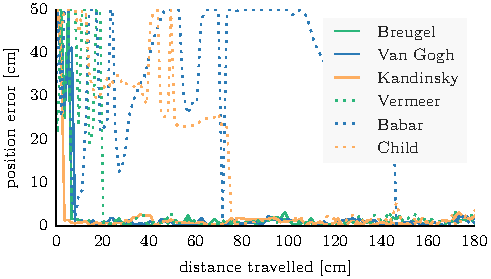
\includegraphics{ml-grayscale_images-random_1-xy}\hfill
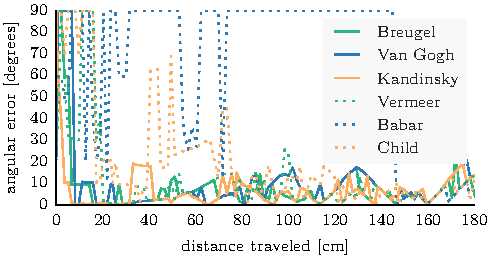
\includegraphics{ml-grayscale_images-random_1-theta}

%\vspace{.3em}

\begin{center}
\texttt{trajectory~2}
\end{center}
\vspace{-.3em}
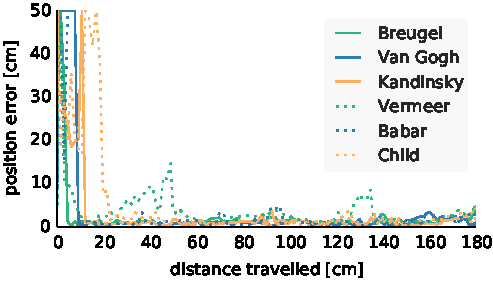
\includegraphics{ml-grayscale_images-random_2-xy}\hfill
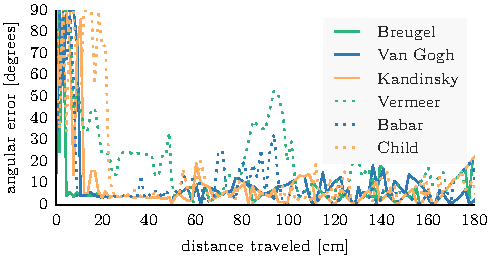
\includegraphics{ml-grayscale_images-random_2-theta}

\caption{The error between the estimation and the ground truth, using Markov Localization with 36 angle discretization, for different grayscale maps.}
\label{fig:grayscale}
\end{figure*}

% FIXME: consider replacing this section with the real-time experiments

In addition to random black and white patterns, our localization model can also work on grayscale images.
While we have not recorded datasets with such images, we simulate these scenarios by using the ground-truth data to look up the corresponding pixel on the image, adding some noise ($\pm$ 0.1, uniform distribution, found using a real Thymio).
When running on such maps, we set $\sigma_\mathrm{obs}$ to 0.1.

\Fig{grayscale} shows the error in position and orientation for six different grayscale maps.
These cover various styles, contrast profiles and distributions of intensities.
The first three, paintings from Breugel, Van Gogh and Kandinsky, allow the robot to localize in less than 10\,cm for both \texttt{trajectory~1} and \texttt{trajectory~2}.
This is due to their variety of contrasted visual structures.
In areas with less contrast, the angular tracking becomes imprecise, but is always within 20°.
The Vermeer painting is harder.
While the robot localizes within 20\,cm on \texttt{trajectory~1}, it has trouble with \texttt{trajectory~2}, especially with the angle.
We attribute this degraded performance to the large areas without contrast in this painting.
The next image is a line-art drawing from a popular children comics.
Stable localization on \texttt{trajectory~1} is only achieved after traveling 150\,cm.
The reason is the low amount of information present in such images.
Nevertheless, when the trajectory encounters sufficient information, like in \texttt{trajectory~2}, accurate localization is possible.
The last image is a child's drawing taken from Wikimedia Commons\footnote{\url{https://commons.wikimedia.org/wiki/File:Child's_Drawing_of_the_Tooth_Fairy.jpg}}.
This drawing allows accurate localization, after traveling 80\,cm in the first run, but only 20\,cm in the second.
This shows that with our model, the robot can localize successfully on maps drawn by children themselves, which opens creative educational opportunities.

\section{Conclusion}

In this paper, we have conducted an empirical evaluation of Markov- and Monte Carlo-based approaches for localizing a mobile robot, equipped with two inexpensive ground sensors, on a known pattern.
We have shown that both approaches allow successful localization without knowing the initial pose of the robot, and that their performances and computational requirements are of a similar order of magnitude.
With current implementations, Markov localization with 36 discretization steps for angle is the most promising choice for deployment in educational activities.
In addition, we have outlined, and empirically validated, a method to estimate the localization performance in function of the sensor configuration.
This method provides a guide for taking decisions about the placement of sensors in a future robot:
localization performance can be improved by placing the sensors far apart on a line perpendicular to the direction of movement of the robot; in addition, more sensors allow for collecting more information, if they are separated by the size of the smallest visual structure in the map.
Finally, we have demonstrated that our model allows successful localization on a large variety of grayscale images, from well-known paintings to drawings made by children.
This opens the way to user-created maps, for instance for a child making a picture with her mobile phone of her own drawing, printing this picture on a poster, and using it as map.

These contributions to the state of the art enable absolute positioning of inexpensive mobile robots costing less than 100\,\$.
In the context of educational robotics, this opens many opportunities in the field of spatial reasoning, but also for art and storytelling.
Hence, by enabling a new range of educational activities, our solution also strongly increases the value of robots for education.

\section{Acknowledgements}

The authors thank Emmanuel Eckard for insightful comments on the manuscript and Ramiz Morina for his drawings.

\bibliographystyle{IEEEtran}
\bibliography{thymio-localisation-iros}

\end{document}



